% sections/04_results.tex
% §4 Results — MS (Lại Minh Dũng, SE194215)

\section{Results}
\label{sec:results}

\subsection*{RQ1: Does Qwen2.5-7B 3-shot reach the GPT-4o reference thresholds?}

The evaluation includes 262 bug reports from the Bugzilla test
set. Table~\ref{tab:results} presents the descriptive
statistics together with the outcomes of the Wilcoxon
signed-rank tests. Figure~\ref{fig:boxplot} illustrates the
distribution of the three evaluation metrics relative to the
corresponding GPT-4o reference thresholds.

\begin{table}[t]
\centering
\caption{Evaluation results of Qwen2.5-7B with 3-shot prompting
on the Bugzilla test set (N=262). The benchmark thresholds are
taken from the GPT-4o 3-shot results reported by
\protect\cite{acharya2025bugquality}.}
\label{tab:results}
\begin{tabular}{lcccccc}
\toprule
\textbf{Metric} &
\textbf{Threshold} &
\textbf{Median} &
\textbf{IQR} &
\textbf{\textit{p}-value} &
\textbf{Cliff's $\delta$} &
\textbf{Decision} \\
\midrule
CTQRS (\%) &
$\geq$75.0 &
88.89 &
[83.33, 94.44] &
$<$0.001 &
0.908 (large) &
Reject $H_0$ \\

ROUGE-1 F1 &
$\geq$0.47 &
0.491 &
[0.420, 0.551] &
0.002 &
0.191 (small) &
Reject $H_0$ \\

SBERT &
$\geq$0.82 &
0.632 &
[0.549, 0.701] &
1.000 &
$-$0.969 (large) &
Fail to reject $H_0$ \\
\bottomrule
\end{tabular}
\end{table}

\textbf{H1.1 -- CTQRS.}

CTQRS values were generally high across the evaluation set.
The median reached 88.89\%, and half of the reports obtained
scores within the interval of 83.33\% to 94.44\%. The reported
median was above the reference value of 75\%.

Statistical analysis using the Wilcoxon signed-rank test
returned $p<0.001$. The corresponding Cliff's $\delta$
was 0.908, representing a large effect size.
Accordingly, $H_0^{\text{CTQRS}}$ was rejected.

Most reports received relatively high CTQRS scores.
Specifically, 89 reports obtained 16 points, 55 obtained
17 points, and another 13 reached the maximum score of
18 points. Only 12 reports (4.6\%) scored below the
reference threshold.

\textbf{H1.2 -- SBERT.}

The SBERT similarity scores are centered around a median of
0.632. The interquartile range extends from 0.549 to 0.701,
which remains below the benchmark value of 0.82.

The statistical comparison resulted in a $p$-value of 1.000,
with Cliff's $\delta$ equal to $-0.969$, indicating a large
effect in the opposite direction. Accordingly,
$H_0^{\text{SBERT}}$ was not rejected.

\textbf{H1.3 -- ROUGE-1.}

ROUGE-1 F1 achieved a median score of 0.491.
The middle half of the observations ranged from
0.420 to 0.551, placing the median above the
reference threshold of 0.47.

The Wilcoxon signed-rank test returned
$p=0.002$, while Cliff's $\delta$ was 0.191,
representing a small effect size.
Therefore, $H_0^{\text{ROUGE-1}}$ was rejected.

\textbf{Bonferroni correction.}

To account for the three hypothesis tests performed for RQ1,
a Bonferroni correction was applied, resulting in an adjusted
significance level of
$\alpha_{\text{adj}}=0.05/3\approx0.017$.The conclusions were unchanged after applying the correction.
CTQRS ($p_{\text{adj}}<0.001$) and ROUGE-1
($p_{\text{adj}}=0.005$) continued to reject the null
hypothesis, whereas SBERT
($p_{\text{adj}}=1.000$) continued to fail to reject it.

\begin{figure}[t]
\centering
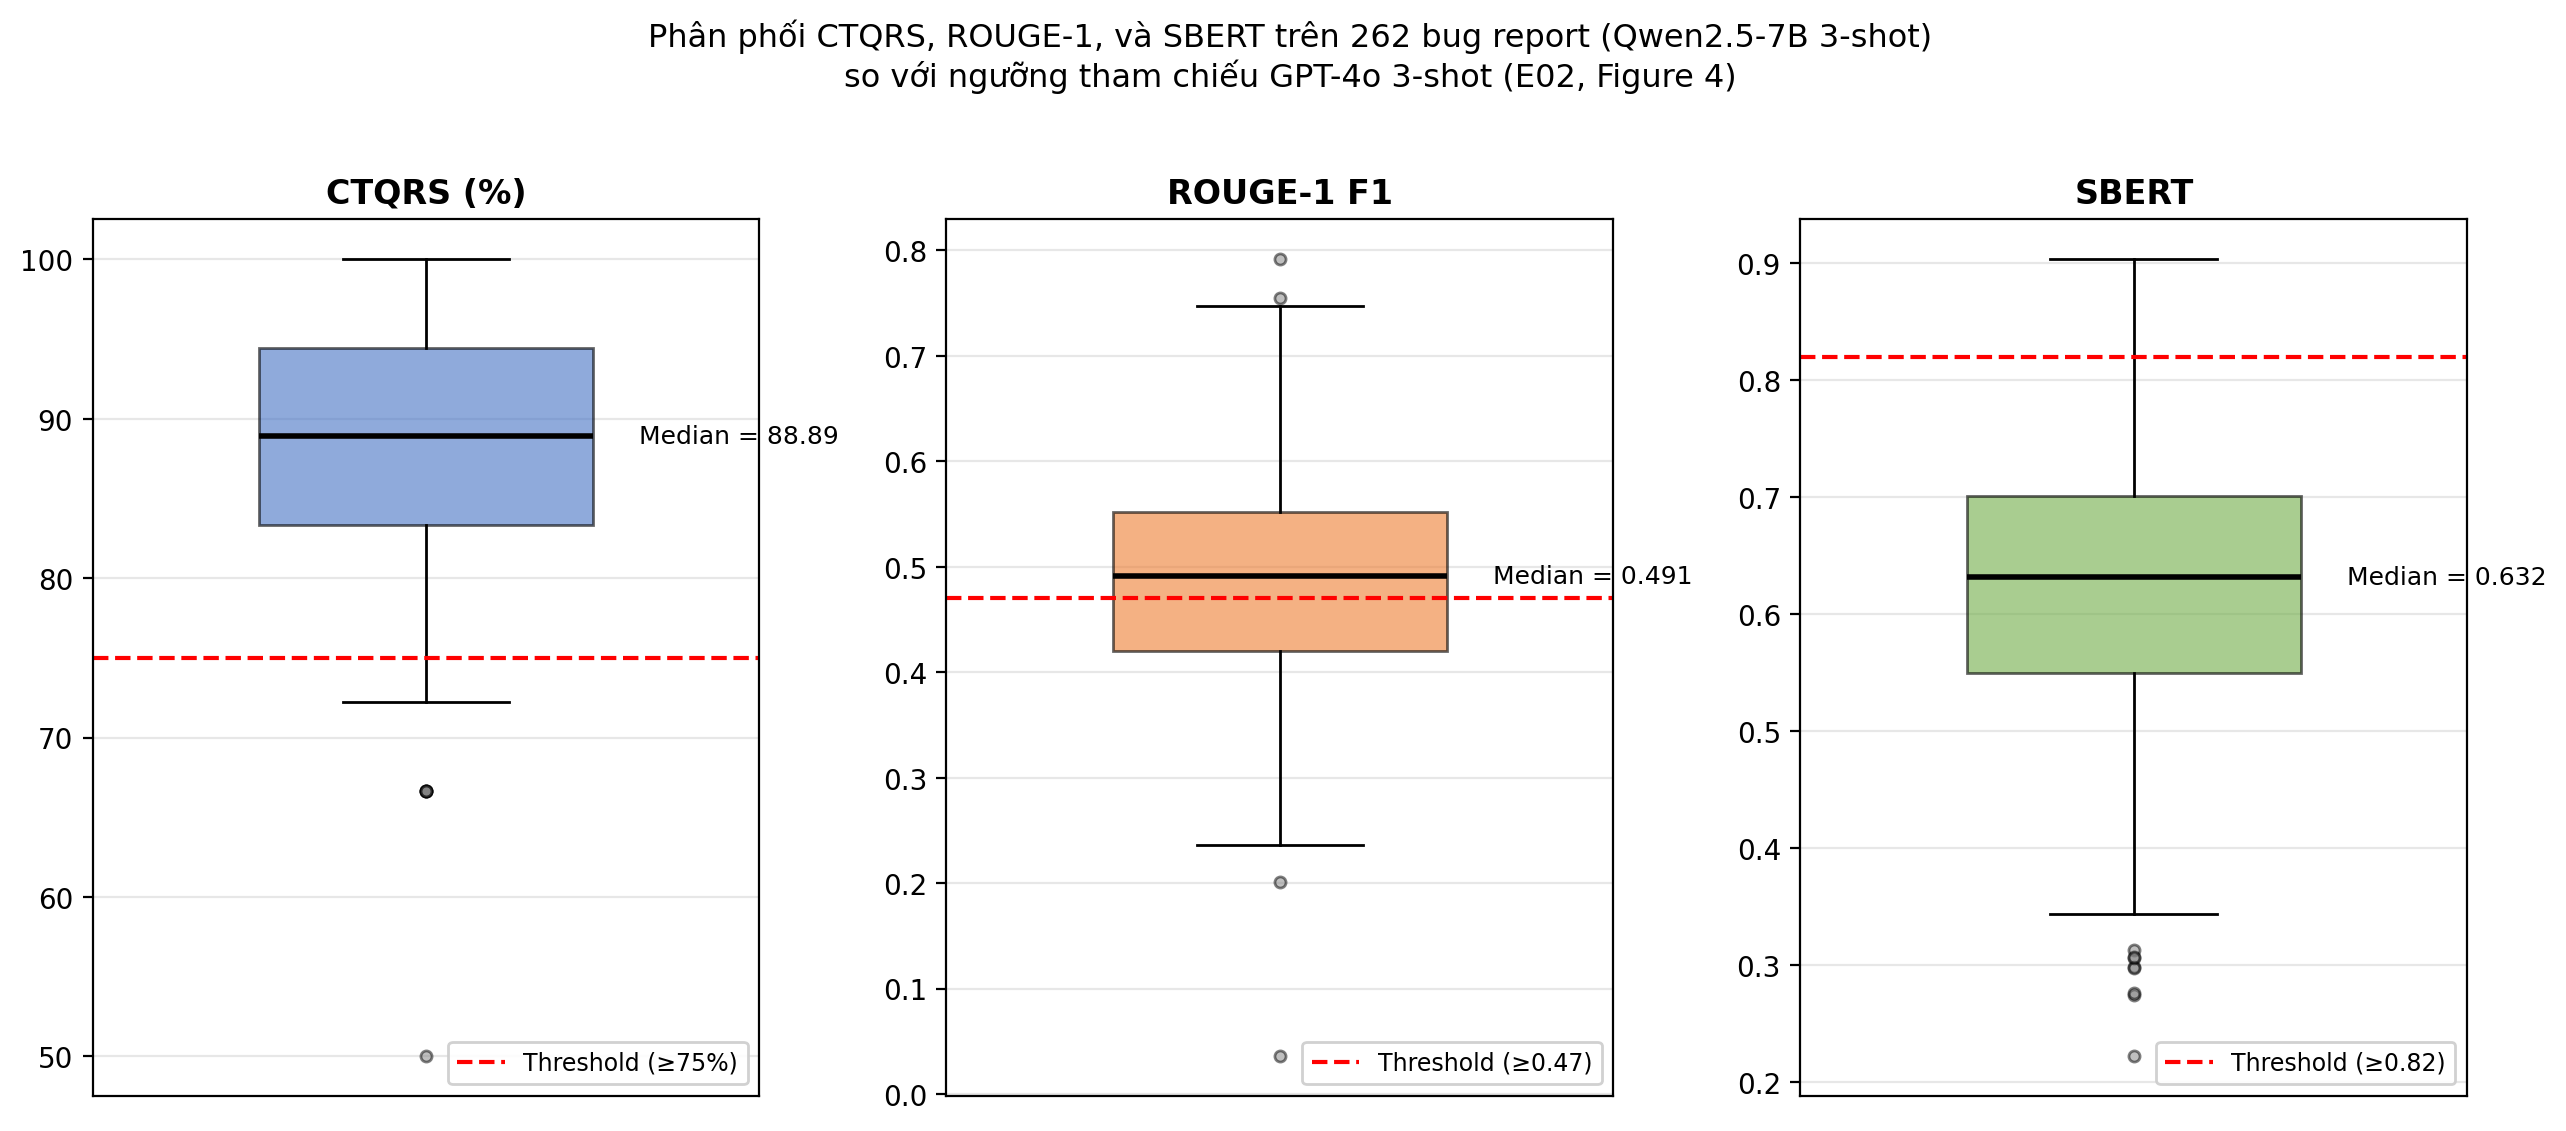
\includegraphics[width=\columnwidth]{figures/figure1_boxplot.png}
\caption{Distributions of CTQRS (\%), ROUGE-1 F1, and SBERT
scores obtained by Qwen2.5-7B with 3-shot prompting
(N=262). The dashed red lines represent the GPT-4o
reference thresholds reported by
\protect\cite{acharya2025bugquality}.}
\label{fig:boxplot}
\end{figure}

\textbf{Overall answer to RQ1.}

Across the three evaluation metrics, Qwen2.5-7B met the
published reference thresholds for CTQRS and ROUGE-1 F1.
However, the observed SBERT scores remained below the
corresponding GPT-4o reference threshold.